%! suppress = UnresolvedReference


\chapter{相关技术介绍}\label{ch:tech}


\section{Flutter跨平台应用程序开发框架}\label{sec:flutter}

\subsection{使用跨平台应用程序开发框架的意义}\label{subsec:why-framework}

要开发一个面向移动终端的\app ,首先要考虑的是该应用支持哪些移动平台。根据2023年3月的数据\cite{MobileOperatingSystem},在中国的移动平台操作系统占有率中,Android系统以76.15\%名列第一,iOS系统以23.28\%位居第二,这两个最主流的移动平台操作系统占据了绝大部分市场份额。因此,本应用开发的目标平台选定为Android和iOS。

Android和iOS开发的各种技术可以分为两大方向:原生应用程序开发和跨平台应用程序开发。构建传统的原生应用程序需要维护两个不同的代码库,分别为Android和iOS平台编写代码,通常意味着需要分别使用Kotlin/Java和Swift/Objective-C来编写两份高度相似的代码。而跨平台应用程序开发框架则可以通过一套代码库同时为Android和iOS平台构建应用程序,降低了开发人员的学习成本,缩减了开发时间,提高了开发效率。

\subsection{Flutter简介}\label{subsec:flutter}

Flutter是一个由Google开源的跨平台应用程序开发框架,仅通过一套代码库就能构建精美的、原生平台编译的跨平台应用\cite{FlutterBuildApps}。

Flutter对Android和iOS平台均有良好支持,此外还支持Windows、Linux、macOS、Web等平台\cite{SupportedDeploymentPlatforms}。基于Flutter框架进行开发不仅可以避免为Android和iOS平台分别编写大量相似的代码,还可以方便未来将部分不依赖于移动端特性的功能(比如历史心电展示等)的相关代码在其他平台(比如Web端)复用。

\subsection{Flutter与其他框架的对比}\label{subsec:flutter-compare}

Flutter并不是唯一一个支持Android和iOS平台的跨平台应用程序开发框架。在本项目的选型过程中也考虑了其他几个经常被与Flutter进行比较的同类框架,包括React Native\cite{ReactNativeLearn}、Xamarin\cite{XamarinOpensourceMobile}、Ionic Creator\cite{IonicFrameworkCrossPlatform}。

关于这几个框架,最先被对比的是其热度。以近一年的Google趋势作为标准,对比结果如图~\ref{fig:google-trends} 所示。

\begin{figure}[h]
    \centering
    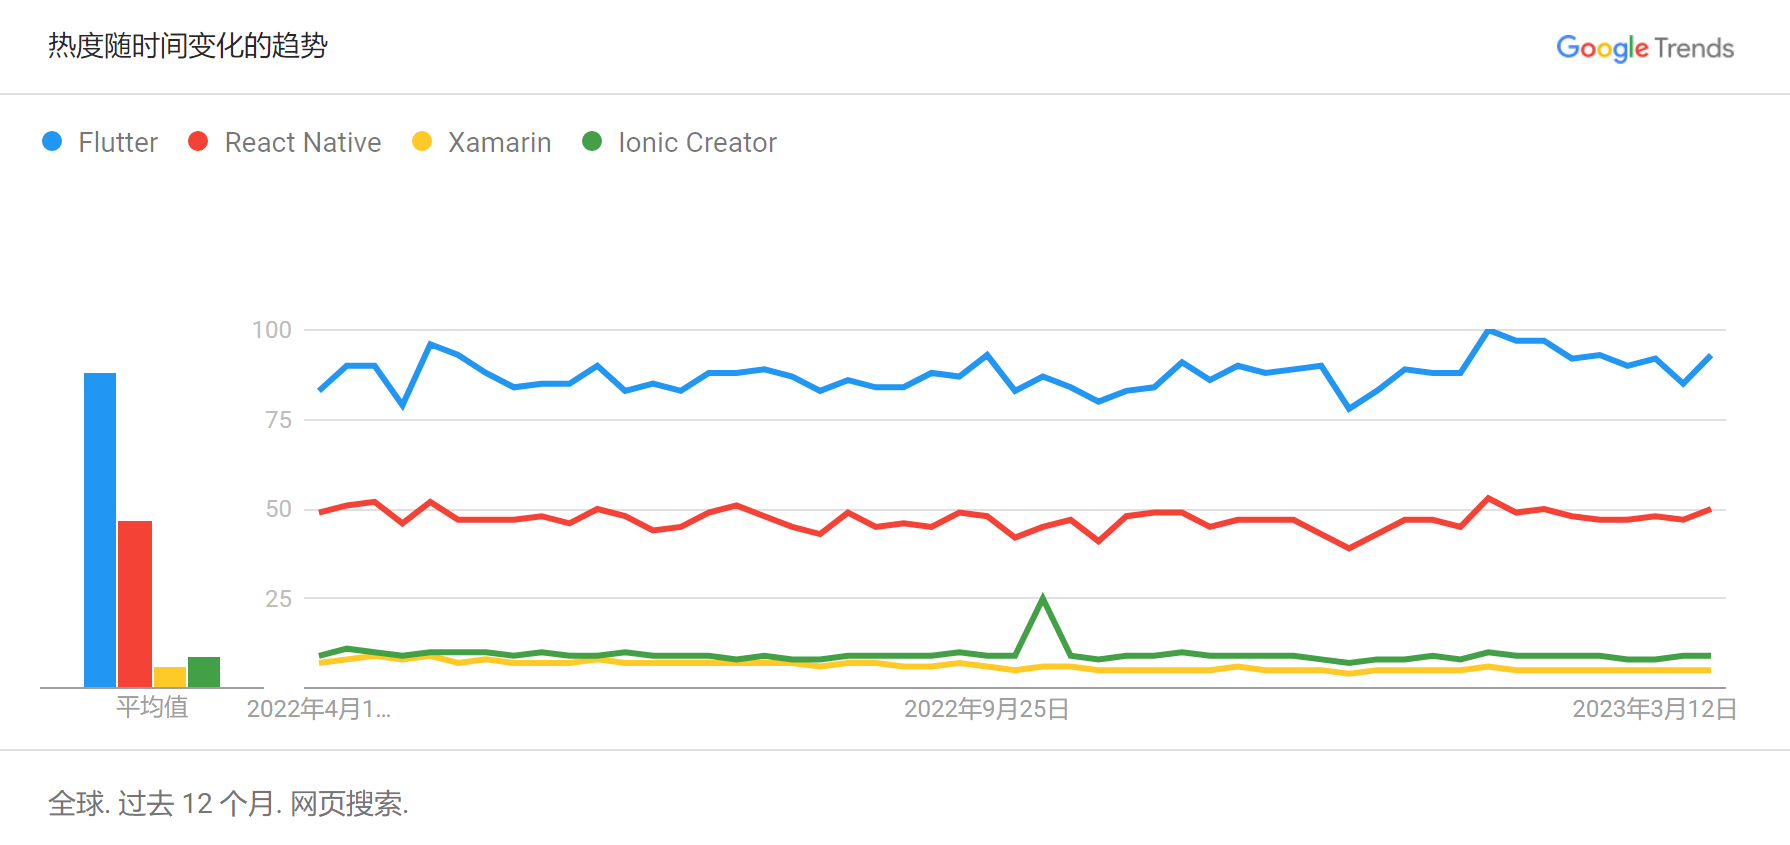
\includegraphics[width=\textwidth]{../assets/google-trends}
    \bicaption{Flutter与其他框架的Google趋势}{Google Trends for Flutter and other frameworks}
    \label{fig:google-trends}
\end{figure}

从图中可以看出,Flutter和React Native的热度远远高于Xamarin和Ionic Creator。热度高意味着其社区更加活跃,生态更为优秀,更容易找到相关的资料和技术支持,也更容易利用社区已经开发过的包,这些对于项目开发来说都是非常重要的。因此,Xamarin和Ionic Creator在本项目的选型过程中最先被排除。

之后需要对比的是Flutter和React Native。从热度上来看,两者的热度都比较平稳,Flutter长期保持在React Native的两倍左右,这意味着Flutter应当被优先考虑,但还不足以作为决定性理由。因此,需要进一步对比这两个框架的特性。

React Native是由Meta(前身为Facebook)于2015年开源的跨平台应用程序开发框架。正如其名称所暗示的,React Native和React(一个流行的Web框架)的关系十分密切,这既是优点也是缺点。从优点的方面来说,React Native非常适合已有React开发经验但没有移动平台开发经验的开发者快速上手,也适合将已有的基于React的Web项目迁移至移动端,但这两点对于本项目来说都没有明显意义。另一方面,由于和React的紧密联系,基于React Native的应用需要使用JavaScript和CSS编写,代码会在JavaScript引擎下解释执行,并通过序列化消息与本机代码桥接通信以渲染原生组件。JavaScript本来就不是一种以性能见长的语言,额外的桥接翻译层更使得其性能较之原生应用程序相去甚远。

作为对比,Flutter是Google于两年后(2017年)开源的,其设计上明显借鉴了React Native,与其一样使用响应式风格的界面编写方式。主要差别在于Flutter是编译成原生代码运行,直接接管并控制屏幕上的每一个像素,由此可以避免使用JavaScript桥接导致的性能问题。

除了上述的性能优势之外,Flutter还在热重载、IDE集成、内置调试工具等方面相较其他框架更为优秀。最终,基于以上所有考虑,本项目选择了Flutter作为开发框架。

\subsection{Dart语言}\label{subsec:dart}

Dart是由Google开源的编程语言,专门针对用户界面(User interface,缩写为UI)的创造进行优化,可编译为移动平台、桌面平台的二进制文件和Web平台的Javascript代码\cite{DartProgrammingLanguage}。Dart最初于2011年发布,原本是打算捆绑于Chrome浏览器来替代JavaScript,但后来由于各种因素而未能成功。在Flutter开发团队选择了Dart作为开发语言之后,两者的关系便愈加紧密,Dart也因此得到了更多的关注,并顺应Flutter框架的需求进行了许多更新迭代。时至今日,Dart与Flutter可以说是处于完全捆绑的状态,基于Flutter框架进行开发几乎是学习并使用Dart语言的唯一目的,使用Dart语言也是基于Flutter框架进行开发的必要条件。

Dart是一种多范式的语言,支持函数式、命令式、面向对象、反射式的写法,语法风格近似于C++与Java的混合,支持抽象类、泛型、类型推断、自动内存管理、空安全等其他语言中较为常见的特性,也有Mixin、Extension方法等其他语言中不太常见的特性。因篇幅限制,本文不便对Dart的诸多特性进行完整介绍,这里仅对后文必须涉及,且与其他语言有明显差异的部分特性进行简单说明。

\subsubsection{外部函数接口}\label{subsubsec:ffi}

外部函数接口(Foreign function interface,缩写为FFI)是一种机制,指用一种编程语言编写的程序可以调用另一种编程语言编写的功能。比如在C++中可以指定 \lstinline[language=C]{extern "C"} 来要求编译器在调用约定、名字重整等方面遵循C语言的标准\footnote{这一特性在C++中被称为语言链接(Language linkage)。},从而实现与C语言之间的双向FFI。

Dart作为一种专精于UI开发的语言,在其他方面的生态较为薄弱。作为一种弥补方式,Dart实现了与许多其他语言之间的FFI,比如在Web上可以与JavaScript互相调用,在macOS和iOS上可以与Swift或Objective-C互相调用,在Android、Windows、macOS、Linux上可以与Kotlin或Java互相调用,以及对本项目来说最重要的——在除Web以外的所有平台可以与C语言直接进行交互,而无须像React Native等框架那样通过Java等中间层进行间接调用,这使得Dart与C语言之间的FFI十分高效。由于C++代码也可以通过指定 \lstinline[language=C]{extern "C"} 来编译为与C语言格式相同的接口,这意味着本应用的部分功能可以直接使用C++编写,从而充分利用C++的性能、生态、跨平台性等优势。

在项目的开发过程中,使用C++编写了两部分代码供Dart FFI调用,分别是Pan-Tompkins算法和基于LibTorch的人工智能算法,在后文会详细介绍。

\subsubsection{Isolate}\label{subsubsec:isolate}

Isolate\footnote{该术语没有常用的中文译名,故本文中直接使用英文原名。}是Dart中的一种介于线程与进程之间的概念。在Dart程序中,所有的代码都在isolate中运行。每一个isolate都有独立的运行线程和独立的堆内存,从而确保isolate之间互相隔离,无法互相访问状态。相比于常规的线程,这样的实现并不会共享内存,所以也不需要担心互斥锁和其他锁等问题。相对地,由于无法与其他isolate共享可变对象,isolate之间的通信必须使用消息机制。

Dart程序有一个默认的主isolate,在Flutter应用中也称为UI isolate,因为UI的更新都是在主isolate中进行的。在本应用中,数据库查询等可能较为耗时的操作都是放在其他isolate中异步执行的,以避免阻塞UI isolate导致UI卡顿。

\subsection{项目使用的Flutter包}\label{subsec:flutter-packages}

尽管Flutter SDK本身已经包含了大量的基础组件,但是在实际开发中,还是经常需要额外使用官方或社区开发的Flutter包来实现一些特定的功能。本项目所使用的Flutter包总计有上百个,其中一些包的使用比较简单,比如URL Launcher包只是用来在各个平台提供在浏览器中打开指定的URL的功能;而另一些包则在项目开发的各个阶段有着广泛的影响,比如Isar包的特性直接影响了本项目数据库的设计、实现与测试。

由于项目使用的Flutter包非常多,而且作用分散在项目的各个阶段、各个模块,在此处一一介绍会使得本节过于冗长且难以理解,本文在后续章节涉及到相关Flutter包时再对各个包分别进行说明。另外,所有包的相关文档均可在 \url{https://pub.dev/} 上找到,由于数目众多,本文不在参考文献中分别列出。


\section{项目使用的Python包与C++中的对应替代}\label{sec:python-cpp-packages}

\subsection{将Python代码迁移至C++的原因}\label{subsec:why-cpp}

本项目使用的用于心电信号分析的人工智能算法最初是使用Python编写的。为了在面向移动终端的应用中使用这些算法,考虑了各种可能的技术方案。

\subsubsection{移动端直接执行Python代码的方案}\label{subsubsec:run-python}

最简单的一个方案是设法在移动端直接执行Python代码。这种方式在移动应用开发中很少被使用,主要是基于时间上和空间上这两个方面的顾虑。从时间上来说,Python语言的执行效率较低,在设备性能相对较差的移动端表现得更为明显;不过本应用中人工智能算法的执行时间占比并不大,仅仅是每10分钟调用一次,一次执行数秒而已,所以这一缺点也并非不可接受。从空间上来说,将Python语言的运行环境打包进应用会导致应用的安装包体积更大;但此算法所需要的Torch模型文件本身就已有60多MB,相较之下Python的运行环境所额外占据的大小并不是很明显。因此,常见的关于性能或安装包大小的顾虑并不能构成否定本方案的充分依据。之后考虑了在移动端执行Python代码的各种方式。

PyQtDeploy\cite{RiverbankComputingIntroduction}、QPython\cite{QPythonPythonAndroid}、Termux\cite{Termux}等工具可以用于在移动端执行Python代码,但未提供可供Java、Dart等语言调用的接口,因此无法在本项目中使用。

Kivy\cite{KivyCrossplatformPython}提供了Python与Java、Objective-C的交互,但是缺少对于PyTorch的支持,而这一依赖难以替代,所以Kivy也无法在本项目中使用。

Chaquopy\cite{EasiestWayUse}提供了PyTorch的支持。尽管最高只支持1.8.1版本,但算法原本所依赖的版本甚至比这更旧,所以PyTorch的使用没有问题。但是,Chaquopy仅支持Android平台,而不支持iOS平台,所以无法完全满足本项目的需求。

BeeWare\cite{WriteOnceDeploy}在Chaquopy之上增加了对iOS平台的支持,但是需要将整个应用都使用Python编写,这样就无法通过仅在少数部分调用Python来避开本小节最初提到的性能问题,因此也不是可行的方案。

综合以上调查结果,可以认定移动端直接执行Python代码的方案并不可行。因此,必须将原本使用Python编写的算法迁移至其他语言。

\subsubsection{使用Dart实现相关算法的方案}\label{subsubsec:python-dart}

由于应用主体使用Dart编写,下一个考虑的方案是使用Dart实现相关算法。社区已经编写了PyTorch Mobile、PyTorch Lite等包来帮助将PyTorch模型迁移至Flutter框架,但这些包都仅支持对模型的直接调用,而本项目所使用的算法除了直接调用模型的部分之外还包含一些额外的处理步骤,这些步骤在缺少相关支持的Dart中较难实现,因此这一方案也不可行。

\subsubsection{使用C++实现相关算法的方案}\label{subsubsec:python-cpp}

\todo{为什么需要C++中的对应替代?(需要将Python算法迁移至C++,部分关键依赖无法消除。)}

本项目的一部分工作是将已有的使用Python编写的算法迁移至C++。

\subsection{PyTorch与LibTorch}\label{subsec:pytorch-libtorch}

\todo{什么是PyTorch?}

\todo{什么是LibTorch?}

\todo{为什么选择LibTorch而不是PyTorch Mobile、MNN、NCNN等?(PyTorch官方支持,接口设计高度相似,引用官方文档中相关说明。)}

\subsection{NumPy与NumCpp}\label{subsec:numpy-numcpp}

\todo{什么是NumPy?}

\todo{什么是NumCpp?}

\todo{为什么选择NumCpp而不是Eigen等?(接口与NumPy更相似。)}

\subsection{pytest与Catch2}\label{subsec:pytest-catch2}

\todo{什么是pytest?(关于名字:pytest的官方名称即为全小写形式,即使在位于句首的情况下也是如此。)}

\todo{什么是Catch2?}

\todo{为什么选择Catch2而不是Google Test、Boost Test等?(更简单,本项目的C++部分没有编写复杂的测试用例的需求。)}

\subsection{nlohmann::json}\label{subsec:nlohmann-json}

\todo{为什么需要nlohmann::json?(Python标准库有JSON支持,C++没有,需要第三方库。)}

\todo{什么是nlohmann::json,不是其他JSON库?(接口简单。虽然性能有劣势,但只是用于读取少量测试数据,速度不重要。)}
